\PassOptionsToPackage{spanish}{translator}
\documentclass{beamer}

\usepackage{etex} % Porque sino al usar muchos paquetes da error.

\usepackage[spanish]{babel}

\mode<presentation> {
\usetheme{Madrid}
}

\usepackage[utf8]{inputenc}
\usepackage{amsmath}
\usepackage{graphicx}
\usepackage{booktabs} % Allows the use of \toprule, \midrule and \bottomrule in tables
\usepackage{multicol}

\usepackage[export]{adjustbox} % Para bordes en las imágenes.

\usepackage{svg}

\usepackage{amsfonts}

\usepackage{array}

\setkeys{Gin}{height=7cm}

\graphicspath{{img/}}

\DeclareMathOperator*{\argmax}{arg\,max}

\title[SRL]{Sistemas para el Etiquetado de Roles Semánticos}

\author[Santiago Castro]{Santiago Castro}
\institute[]{
    Curso de Análisis Semántico de Lenguaje Natural de Dina Wonsever
}
\date{22 de diciembre de 2016}

\usepackage{pgfpages}

\begin{document}

\begin{frame}
    \titlepage{}
\end{frame}

\begin{frame}
  \frametitle{Repaso}

  \begin{itemize}
    \item \textit{Juan le compró el diario a su madre.}

    \begin{itemize}
      \item Agente: Juan
      \item Tema: el diario
      \item Beneficiario: a su madre
    \end{itemize}
  \end{itemize}
\end{frame}

\begin{frame}
  \frametitle{Motivación}

  \begin{itemize}
    \item Identificar y clasificar entidades relacionadas a un predicado.

    \item \textit{Juan compró el diario por \$50.}

    \begin{itemize}
      \item ¿Quién compró?
      \item ¿Qué se compró?
      \item ¿Por cuánto?
    \end{itemize}

    \item Sirve como entrada para otras tareas.
  \end{itemize}
\end{frame}

\begin{frame}
  \frametitle{Roles}

  Podemos definir un conjunto ``estándar''.

  \begin{itemize}
    \item Agente
    \item Paciente
    \item Tema
    \item Experimentante
    \item Beneficiario
    \item Instrumento
    \item Lugar
    \item Origen
    \item Destino
  \end{itemize}

  Pero es ambiguo: \textit{La tormenta derribó la cerca.}
\end{frame}

\begin{frame}
  \frametitle{Proto-roles}

  \begin{itemize}
    \item Si se parece a un Agente, lo es. Similar para Paciente.

    \item PropBank sigue este esquema verbo a verbo, con las mismas etiquetas. Los roles para Arg0 y Arg1 están bastante claros, pero para el resto no se puede hacer una generalización.
  \end{itemize}
\end{frame}

\begin{frame}
  \frametitle{Roles por clases de predicados}

  \begin{itemize}
    \item Los verbos se agrupan en clases y se definen roles para cada uno de ellos.

    \item VerbNet sigue este enfoque.

    \item Además hay problemas por la dispersión de los datos (pocos ejemplos de cada clase para aprender).

    \item ¿Qué pasa si al querer analizar hay un verbo fuera del vocabulario?

    \item Hay que identificar la clase de un predicado a la hora de analizar.

    \item Por otro lado los argumentos de una misma clase pueden tener poco sentido.
  \end{itemize}
\end{frame}

\begin{frame}
  \frametitle{Roles según situaciones}

  \begin{itemize}
    \item FrameNet distingue ``situaciones'' y les asocia predicados.

    \item Tienen roles asociados.

    \item Más problemas de dispersión.
  \end{itemize}
\end{frame}

\begin{frame}
  \frametitle{Semlink}

  Intenta vincular los proyectos anteriores para interoperabilidad.
\end{frame}

\begin{frame}
  \frametitle{CoNLL}

  Esta tarea fue parte de las ``shared tasks'' de la CoNLL\@ (en base a los roles de PropBank):

  \begin{itemize}
    \item 2004: SRL en inglés, basado en chunking.
    \item 2005: SRL en inglés, con árboles sintácticos provistos.
    \item 2008: Tarea conjunta en inglés de análisis sintáctico y semántico.
    \item 2009: Tarea conjunta multilenguaje de análisis sintáctico y semántico.
  \end{itemize}

  Variantes: con o sin recursos externos.
\end{frame}

\begin{frame}
  \frametitle{CoNLL04}

  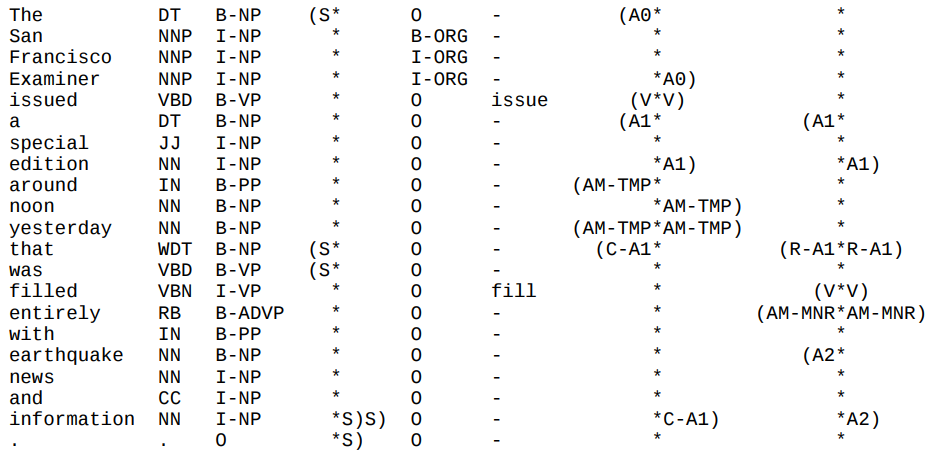
\includegraphics[height=5.7cm]{conll04.png}
\end{frame}

\begin{frame}
  \frametitle{CoNLL09}

  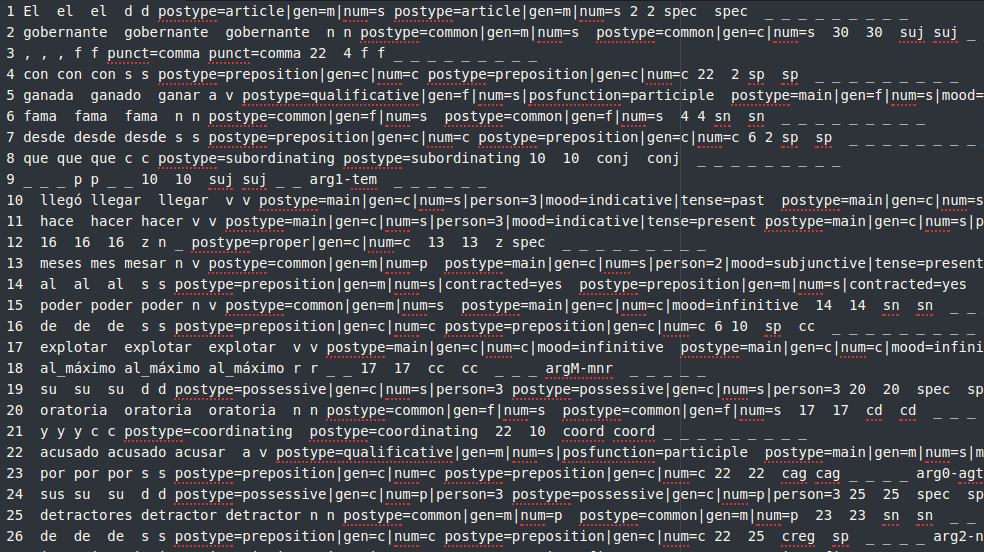
\includegraphics[height=6.7cm]{conll09.png}
\end{frame}

\begin{frame}
  \frametitle{Enfoque}

  Los sistemas en general siguen el siguiente enfoque:

  \begin{enumerate}
    \item Obtener una representación sintáctica de la oración.
    \item Identificar los predicados.
    \item Identificar los argumentos de cada uno.
    \item Calcular features.
    \item Clasificarlos mediante aprendizaje supervisado.
  \end{enumerate}

  Estos sistemas se basan fundamentalmente en una fuerte ingeniería de features.
\end{frame}

\begin{frame}
  \frametitle{Representación sintáctica}

  \begin{itemize}
    \item Árboles de constituyentes o de dependencias.

    \item La calidad del análisis sintáctico va a limitar el etiquetado de los roles.
  \end{itemize}
\end{frame}

\begin{frame}
  \frametitle{Identificación de predicados}

  Se identifican los predicados que aparecen a partir del análisis sintáctico y se procesa cada uno de ellos.
\end{frame}

\begin{frame}[allowframebreaks]
  \frametitle{Identificación de argumentos}

  \begin{itemize}
    \item Se usan heurísticas para luego facilitar la clasificación.

    \item Un algoritmo (Xue y Palmer, 2004): comenzar desde el nodo del predicado del árbol, agregando los nodos hermanos y subiendo hasta encontrar una coordinación o la raíz.

    \item Se prioriza el recall frente a la precisión para evitar restringir la clasificación.
  \end{itemize}

  \framebreak{}

  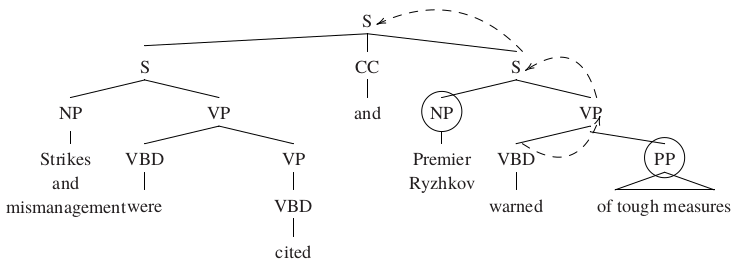
\includegraphics[height=4.4cm]{identificacion.png}
\end{frame}

\begin{frame}
  \frametitle{Features}

  Para hacer clasificación multiclase (una clase para cada tipo de atributo) se han usado distintas features.

\end{frame}

\begin{frame}
  \frametitle{Features}
  \framesubtitle{Tipo de sintagma}

  A partir del árbol se puede saber qué tipo de sintagma es. Como referencia, los elementos de FrameNet se expresan como:

  \begin{itemize}
    \item 47\% nominales
    \item 22\% preposicionales
    \item 4\% adverbiales
    \item \ldots
  \end{itemize}

\end{frame}

\begin{frame}
  \frametitle{Features}
  \framesubtitle{Categoría dominante}

  \begin{itemize}
    \item Para el caso de los sintagmas nominales detectados, puede tener sentido mirar si están dentro de un S o un VP en el árbol. Esto indica con mucha probabilidad si son sujeto u objeto.
    \item Los sintagmas nominales que son sujetos tienen más probabilidad de ser el agente por ejemplo.
  \end{itemize}
\end{frame}

\begin{frame}
  \frametitle{Features}
  \framesubtitle{Camino en el árbol}

  \begin{itemize}
    \item El camino en el árbol desde el predicado al argumento indica con más precisión que la característica anterior el tipo de relación sintáctica.
    \item VB $\uparrow$ VP $\downarrow$ PP\@: argumento o adjunto
    \item VB $\uparrow$ VP $\downarrow$ NP\@: objeto
    \item Aunque hay muchas posibles combinaciones (problemas de dispersión).
  \end{itemize}
\end{frame}

\begin{frame}
  \frametitle{Features}
  \framesubtitle{Posición}

  \begin{itemize}
    \item Posición del argumento respecto al predicado (si está antes o después).

    \item Por ejemplo, el agente tiende a estar antes.
  \end{itemize}
\end{frame}

\begin{frame}
  \frametitle{Features}
  \framesubtitle{Voz pasiva}

  \begin{itemize}
    \item Si es voz activa o pasiva.

    \item Puede condicionar al atributo anterior.
  \end{itemize}
\end{frame}

\begin{frame}
  \frametitle{Features}
  \framesubtitle{Núcleo}

  \begin{itemize}
    \item Algunos núcleos tienden a tener determinados roles.
    \item ``Pedro'' tiene más probabilidad de ser un agente que ``historia''.
  \end{itemize}
\end{frame}

\begin{frame}
  \frametitle{Features}
  \framesubtitle{Ordinal}

  Número de posición del argumento.
\end{frame}

\begin{frame}
  \frametitle{Features}
  \framesubtitle{Otras}

  \begin{itemize}
    \item PoS del núcleo.

    \item Si aparecen entidades con nombre.

    \item Rol del argumento previo.
  \end{itemize}
\end{frame}

\begin{frame}
  \frametitle{Clasificación}

  \begin{itemize}
    \item Autores han usado SVM, kNN, regresión logística, entre otros.

    \item Principalmente procesan los argumentos de forma secuencial.
  \end{itemize}
\end{frame}

\begin{frame}
  \frametitle{Resultados}

  En general se obtiene de $F_1$:

  \begin{itemize}
    \item $\sim$80\% si se cuenta con el análisis sintáctico
    \item $\sim$70\% si se tiene un shallow parsing y las oraciones segmentadas
    \item $\sim$60\% si sólo se tiene un shallow parsing
  \end{itemize}

  Se mide por argumento (en alcance y etiqueta).
\end{frame}

\begin{frame}
  \frametitle{Programación Lineal Entera}

  \begin{itemize}
    \item Otra forma de resolver el problema ha sido con Programación Lineal Entera.

    \item Se ve el problema como una forma de asignar roles a argumentos y se asignan pesos en base a puntajes de un clasificador.
  \end{itemize}
\end{frame}

\begin{frame}
  \frametitle{Tarea conjunta}

  \begin{itemize}
    \item Obtener el análisis sintáctico y semántico.

    \item Da peores resultados que atacando solamente SRL\@.
  \end{itemize}
\end{frame}

\begin{frame}
  \frametitle{Tarea conjunta}
  \framesubtitle{Zhao en CoNLL 2008}

  \begin{itemize}
    \item Obtiene primero un árbol de dependencias usando una versión mejorada del algoritmo de Nivre.

    \item Luego ataca SRL usando el árbol completo lo menos posible, para evitar arrastrar error.

    \item Introduce una forma creativa de identificar los predicados: mirar los pares de palabras relacionados en donde la palabra que gobierna sea verbo o sustantivo. Luego usa el algoritmo de Xue y Palmer para obtener los argumentos.
  \end{itemize}
\end{frame}

\begin{frame}
  \frametitle{Multilenguaje}

  \begin{itemize}
    \item Para el caso de atacar muchos lenguajes, autores han usado las mismas técnicas entrenando múltiples clasificadores.

    \item Hay que tener en cuenta que hay ciertas cosas que miden las características que son específicas al lenguaje. Como el lugar del sujeto en el predicado, o el camino desde el predicado a un argumento.
  \end{itemize}
\end{frame}

\begin{frame}
    \Huge{\centerline{¿Preguntas?}}
\end{frame}

\end{document}
